\chapter{黑洞物理}\label{chpt:BH}

\section{经典实验验证}

黑洞是广义相对论提出之后,第一个也是最重要的研究课题。百年来围绕着黑洞的研究,使我们对相对论、引力、量子场论、统计物理都有了崭新的认识。
而自 Einstein 论文发表以来,对广义相对论的若干实验验证相继提出,其中最为著名的是引力红移、水星进动和星光偏折。

\subsection{引力红移}



考虑等效原理。

假设有一光源在 $r$ 处发出频率为 $\nu$ 的光子,若此时光源静止于某惯性系,则光子能量为 $E=h\nu$。若此时光源以速度 $v$ 沿径向运动,则能量变为
\[E'=h\nu\sqrt{1-v^2/c^2}.\]
若光子在 $r$ 处被接收,且接收器静止于同一惯性系,则光子能量仍为 $E=h\nu$。因此,光子在 $r$ 处的频率为
\[\nu'=\frac{E'}{h}= \nu\sqrt{1-v^2/c^2}.\]
若光源和接收器处于不同的引力场中,设光源在 $r_1$ 处,接收器在 $r_2$ 处,则光子能量为
\[E=h\nu\sqrt{1-2GM/r_1c^2},\]
接收器处的能量为
\[E'=h\nu\sqrt{1-2GM/r_2c^2}.\]
因此,光子在 $r_2$ 处的频率为
\[\nu'=\frac{E'}{h}= \nu\sqrt{\frac{1-2GM/r_2c^2}{1-2GM/r_1c^2}}.\]
这就是引力红移的公式。若 $r_1=r_2$,则 $\nu'=\nu$,即光子频率不变;若 $r_1<r_2$,则 $\nu'<\nu$,即光子频率降低;若 $r_1>r_2$,则 $\nu'>\nu$,即光子频率升高。

引力红移的实验验证是通过测量光子频率的变化来实现的。最著名的实验是 Pound-Rebka 实验,该实验在 1959 年由 Robert Pound 和 Glen A. Rebka 在哈佛大学进行。他们使用了一个高塔和一个伽马射线源,测量了从塔顶到塔底的伽马射线频率变化,验证了引力红移的预测。

\subsection{水星进动}

\begin{wrapfigure}{r}{3cm}\centering
    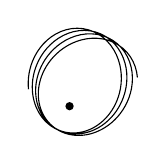
\begin{tikzpicture}[scale=.5]
    \draw[domain=0.4*180/pi:21.6*180/pi,samples=300] plot ({cos(\x)/(1-0.5*cos(0.97*(\x-45)))},{sin(\x)/(1-0.5*cos(0.97*(\x-45)))});
    \fill (0,0) circle(3pt);
    \end{tikzpicture}
    \caption{\small 轨道进动(离心率和进动角均夸大)}
\end{wrapfigure}

19 世纪末,水星近日点进动现象被首次观测。毫无干扰的情况下,Newton 理论当然不能解释进动,因此必须要考虑其它因素,如同当年从天王星轨道扰动发现的“笔尖下的行星”海王星那样。由于地球自转轴的进动,从地球上观测水星的进动大部分是参考系的视觉效果,即岁差,我们直接扣除它。其它因素就是其余行星造成的摄动、太阳实际形状以及广义相对论相应。

先研究摄动。参见 Goldstein《经典力学》第 5$\sim$8 章。
以太阳为参考,水星所处的外引力场写作
\[\bm F(r,t)=\bm F_\odot+\bm F_p=-\frac{{G{M_\odot}m}}{r^3}\bm r-Gm\sum_i\frac{M_i(\bm r-\bm R_i)}{|\bm r-\bm R_i|^3},\]
前一项是太阳的贡献,后面是各行星的作用总和。现在研究后者。设 $\bm r,\bm R_i$ 夹角 $\theta_i$,则 $d_i=|\bm r-\bm R_i|=R_i^2(t)+r^2-2R_i(t)r\cos\theta_i(t)$。
忽略其余行星轨道的离心率之影响,即假定做半径 $\bm R_i$ 的圆周运动。设单个行星角速度为 $\omega_i$,将 $\bm F_p$ 在时域上做 Fourier 展开
\[
\bm F_p=- Gm\sum_i \sum_{n\in\Z} {{a_n}(r){\e^{\i n{\omega_i}t}}}\frac{\bm r-\bm R_i}{|\bm r-\bm R_i|},\quad a_n=\frac{\omega_i}{2\pi}\int_0^{2\pi/\omega_i}{\frac{{M_i\e^{-\i n\omega_i t}\,\d t}}{{R_i^2 + r^2 - 2R_ir\cos \theta_i}}}.
\]
只保留最低阶的 $n=0$ 并用$\d\theta_i$ 替换$\omega_i\d t$ 就可使引力势同时间无关,得到近似表达
\eq{\bm F_p(r) = - Gm\sum_i  \int_0^{2\pi } \frac{M_i\,\d\theta/2\pi}{R_i^2 + r^2 - 2{R_i}r\cos \theta  }\frac{\bm r-\bm R_i}{|\bm r-\bm R_i|},}
引入线密度 $\lambda_i=M_i/(2\pi R_i)$,并沿水星初始方向为极轴,在黄道面上建立极坐标系 $(r,\theta)$,便发现上式表明,其余行星对水星的作用相当于 $M_i$ 均匀分布的一个圆环。这符合直觉,毕竟水星的进动极为缓慢,完整进动一周所需时间相较于其它行星周期很长,因此其它行星的作用的确和圆环类似。但对离水星较近的行星(比如金星),二者周期将在同一数量级,因此不便于近似为圆环。可见圆环模型成立条件是 $R_i\gg r$。幸好,除金星外其它行星都离得较远,将金星视作圆环的影响并不致命。问题现在相当于,在太阳引力基础上,计算附加这样一个微扰后行星的进动。
由圆环对称性,可知作用力与 $\bm r$ 同向,即
\[
\bm F_p= Gm\frac{\bm r}{r}\sum_i  \lambda_iR_i\int_0^{2\pi } \frac{\cos\alpha\,\d\theta}{ d_i^2},
\]
可见其他引力的作用可视作朝外的有心力,我们就可直接讨论分量 $F=F_\odot+F_p$。
我们希望先计算出 $F_p$ 与 $r$ 的关系,虽无初等表达,但由于该式本身就具条件 $R_i\gg r$,故可近似计算。一个聪明的做法并非按 $r/R_i$ 展开,而是重构模型本身。将 $(r,\theta)$ 平移以使原点与水星重合,记新坐标 $(d,\alpha)$,则 $R_i^2=r^2+d_i^2+2rd_i\cos\alpha$,
由于 $\alpha=0$ 时 $d_i=R_i-r$,取解 $d_i=-r\cos\alpha+\sqrt{R_i^2-r^2\sin^2\alpha}$。
由 $R_i\gg r$ 知圆环可近似看作按 $\alpha$ 均匀分布,故 $ R_i\d\theta\approx d_i\d\alpha$,于是
\begin{align*}
    \int_0^{2\pi } \frac{R_i\cos\alpha\,\d\theta}{ d_i^2 }&\approx \int_0^{2\pi } \frac{\cos\alpha\d{\alpha}}{-r\cos\alpha+\sqrt{R_i^2-r^2\sin^2\alpha}}\\
    &=\int_0^{\pi } \left(\frac{\cos\alpha\d{\alpha}}{-r\cos\alpha+\sqrt{R_i^2-r^2\sin^2\alpha}}-\frac{\cos\alpha\d{\alpha}}{r\cos\alpha+\sqrt{R_i^2-r^2\sin^2\alpha}}\right)\\
    &=\frac{2r}{R_i^2-r^2} \int_0^{\pi }\cos^2\alpha\d{\alpha}=\frac{\pi r}{R_i^2-r^2},
\end{align*}
即
\eq{
F_p=Gm\pi r\sum_i \frac{\lambda_i}{R_i^2-r^2}.
}

接下来只以初始位置 $(r_0,0)$ 为极轴方向建立极坐标,以研究水星运动。有心力的形式为
$m(\ddot r-\dot\theta^2r)=F(r), 2\dot r\dot\theta+\ddot\theta r=0$。第二式导致角动量守恒,记 $mr^2{\dot \theta}=L$。在力学课学过如何从两式消 $t$ 得 Binet 式
\eq{
\dv[2]{\mu}{\theta}+\mu=-\frac{mF}{L^2\mu^2}=J(\mu),\quad \mu=1/r.
}
默认加入微扰前是圆轨道模型,则 $\dv*{\mu}{\theta}=0,F_0=-{L^2}/{(mr_0^3)}$,从而 $\mu_0=J(\mu_0)$。
然而圆轨道闭合而不一定稳定。稳定即是说,物体运动受到微扰后依然束缚在圆轨道附近。下面寻找稳定条件。在 $\mu_0$ 附近展开 $J(\mu)$,记 $x=\mu-\mu_0$,只保留至一阶可得波动方程
\[
\dv[2]{x}{\theta}+\left(1-\eval{\dv{J}{x}}_{0}\right)x=0.
\]
如果括号为负,$x$ 将随 $\theta$ 指数增长或衰减,显然不再稳定。因此稳定要求括号为正,则 $x$ 将随 $\theta$ 作周期振荡。代入 $J(\mu)$ 定义得
\[\eval{\dv{J}{x}}_{0}=\eval{\dv{\mu}}_{\mu_0}\left(- \frac{mF}{L^2\mu^2} \right)= \frac{2m}{L^2\mu_0^3}F_0 - \frac{m}{L^2\mu_0^2} \eval{\dv{F}{\mu}}_{\mu_0} = -2 - \frac{r_0}{F_0} F'(r_0).\]
这里撇号表示对 $r$ 求导。则稳定轨道要求有心力的形式满足
\eq{
1-\eval{\dv{J}{x}}_{0}=3+\frac{r_0}{F_0} F'(r_0)>0.
}
在波动方程中,这个括号的含义是频率平方,注意其中是对 $\theta$ 求导而非 $t$,故应是
\[
\frac{2\pi}{\Delta\theta}=\sqrt{3+\frac{r_0}{F_0} F'(r_0)}.
\]
其中 $\Delta\theta$ 的含义就是一次微扰振荡周期
\[
T_r=\frac{\Delta\theta}{\dot\theta}=\frac{\Delta\theta mr_0^2}{L}=\Delta\theta\sqrt{-\frac{F_0}{mr_0}}
\]
所扫过的角度。可见只有 $F_\odot$ 时使 $\Delta\theta=2\pi$,相当于又回到原位而无进动。而一旦错开,一次周期内就出现了进动。代入数据知
\eq{
r_0F_p'(r_0)=Gm\pi r_0 \sum_{i=2}^9 \lambda_i\frac{R_i^2+r_0^2}{(R_i^2-r_0^2)^2}\approx 1.088 \times 10^{16}\,\mathrm{N},
}
而 $F_p(r_0)\approx 7.587 \times 10^{15}\,\mathrm{N}, F_\odot(r_0)\approx -1.318 \times 10^{22}\,\mathrm{N}$。代入 $F=F_{\odot}+F_p$ 于 $\Delta\theta$ 则\footnote{为更便于计算,还可注意 $F_p(r_0)\approx r_0 F_p^{\prime}(r_0) \ll |F_\odot(r_0)|$,则展至 $F_p(r_0) / F_\odot(r_0)$ 和 $F_p^{\prime}(r_0) / F_\odot(r_0)$ 的一阶。}
\eq{
\Delta \theta=2\pi\sqrt{\frac{F_{\odot}(r_0)+F_p(r_0)}{F_\odot(r_0)+3F_p(r_0)+r_0F_p'(r_0)}}\approx 2\pi(1+9.884\times 10^{-7}).
}
进动率为
\eq{
\omega=\frac{\Delta\theta-2\pi}{T},
}
式中 $T$ 为水星公转周期,一般取恒星年(sidereal year)\footnote{某行星的恒星年是太阳在黄道上的视位置相对遥远恒星变化一周所经历时间,也相当于该行星相对于遥远恒星公转一周所经历的时间。千禧年时地球恒星年的平均长度为 365.25636 天。回归年(tropical year)是太阳的平黄经变化一周所经历时间。由于太阳视运动非均匀,选取不同的起点会得到不同的长度。若选取春分点作为基准,太阳从春分点出发运行一周再次回到春分点的时间为春分点年。千禧年时回归年的平均长度为 365.24219 天。恒星年比回归年要长 20 分 24.5 秒,这个差异正是地球造成的岁差。},或甚至是 $T_r$,再不济用 Kepler 第二定律计算亦可。代入数据知
\[\omega\approx\frac{\pi(1.977\times 10^{-6})}{87.969\,\text{天}}\approx 532''/\text{世纪},\]
仍与观测值 $575''$/世纪相差 $43''$/世纪。

再考虑广义相对论效应。

通过求解在所谓的\textit{线性近似}下的场方程,就可以算出水星近日点进动的正确值。只要能够取得这个进动的正确值,就表示广义相对论的正确性已经通过了该实验的检验。



\subsection{星光偏折}
Eddington(1882-1944,英国天体物理学家) 在 1919 年的一次日食观测中摄下了光线被引力“弯曲”的图片。这一点已经在几何光学近似中从理论上计算过。从那以后,用太阳系的种种检验对场方程作了所谓的,这些预测和实验都在这个物理条件下以很高的精度证实了广义相对论.

如果我们考虑黑洞附近的光线,一路走向测地线方程,所描述的轨迹曲线可以作为\textit{引力透镜(gravitational lensing)}的定量解释。

\subsection{后 Newton 理论}

(post-Newtonian theory)

\section{时空延拓}

\subsection{Eddington 系}

注意到内向族分别在 $r>2M,0<r<2M$ 单调,可设想直接将其映射为向内 $45^\circ$ 斜率的直线 $\tilde t=-r+C$,且为了 $r=0$ 时 $t=\tilde t$,可取
\eq{
    \tilde t=t+2M\ln\abs{\frac{r}{2M}-1}.
}
则度规表为
\eq{
\d s^2=-\left(1-\frac{2 M}{r}\right) {\d \tilde t}^2+\frac{4M}{r}\,\mathrm{d} \tilde t\, \mathrm{d} r+\left(1+\frac{2 M}{r}\right)\d r^2,
}
$g_{01}\geqslant 0$ 符合黑洞演化的方向。现在度规分量在视界处收敛,且 $g=-(g_{01})^2\ne 0$,这才算消去奇性。


$t=-r_*+C$,且为了 $r=0$ 时 $r_*=0$,可取
\eq{
    r_*=r+2M\ln\abs{\frac{r}{2M}-1}.
}
类比 Zeno 悖论\footnote{古希腊哲学家 Zeno 描述了类似效应:运动员 Achilles 欲同一只乌龟赛跑,且乌龟起点先于他若干路程 $L$。按通常的时间 $t$ 来说,他的速度 $v_1$ 快于乌龟的 $v_2$,明显在有限时间 $t=L/(v_1-v_2)$ 内超过乌龟。但设想这样计时:他欲超过乌龟,必须先追至乌龟的起点,但一旦如此,乌龟又能前进若干步,这样便有新的起点等着他,如此这般有无穷多这样的起点,则他“永远”也赶不上乌龟。这种计时方法称为 Achilles 时或 Zeno 时,记作 $t'$。令 $t',t$ 皆起于零。当 $t=L/v_1$ 时,Achilles 到达乌龟在 $t'=0$ 时的起点, $t'$ 加一,以此类推有
\[t=\sum_{i=0}^{t'-1} \frac{L}{v_1}\left(\frac{v_2}{v_1}\right)^{i}=\frac{L}{v_1-v_2}\bigg(1-\bigg(\frac{v_2}{v_1}\bigg)^{t'}\bigg)\To t'=\frac{1}{\ln(v_2/v_1)}\ln\left(1-\frac{v_2-v_1}{L}t\right),\]
其中将 $t'\in\N$ 自然延拓至 $t'\in\R_+$。可见 $t'$ 在 $t=L/(v_2-v_1)$ 发散,因此按 $t'$ 衡量他永不超过乌龟。},
可称\textbf{乌龟坐标}(tortoise coordinates)。数学中的 Lambert 函数定义为满足 $x=y\e^y,y\geqslant -1$ 的$y=\operatorname{W}(x)$。用它可解出 $r=2M(1+\operatorname{W}(\pm\e^{r_*/2M-1}))$,正负号对应 $\sgn(r-2M)$。
注意 $\d r_*={\d r}/{(1-2M/r)}$,从而度规表为 $\d s^2=(1-2M/r)\left(-\d t^2+\d r_*^2\right)$,奇性消除了。关键在于,新坐标系给视界赋予发散坐标,就可将度规奇性隐藏起来。

但这个变换还不够,因为行列式 $g$ 在 $r=2M$ 为零。

时间也需要变换。

变换 $x'=x+(r_*-r)$ 在 $r<2M$ 时 $x'<x$,故称\textbf{超前}(advanced)变换,而 $x'=x-(r_*-r)$在 $r<2M$ 时 $x'>x$,故称\textbf{推迟}(retarded)变换。

该坐标系称为\textbf{超前 Eddington–Finkelstein 系},简称 Eddington 系。



利用十字相乘法可分解出两个类光测地线族,其一是
\eq{
\dv{\tilde t}{r}=\frac{r+2M}{r-2M}\Rightarrow \tilde t=r+4M\ln\abs{r-2M}+C_1, \quad r=2M,
}
其二是
\eq{
\dv{\tilde t}{r}=-1\Rightarrow \tilde t=-r+C_2.
}
显然前者为外向族而后者为内向族。
\begin{figure}[h!]
    \centering
    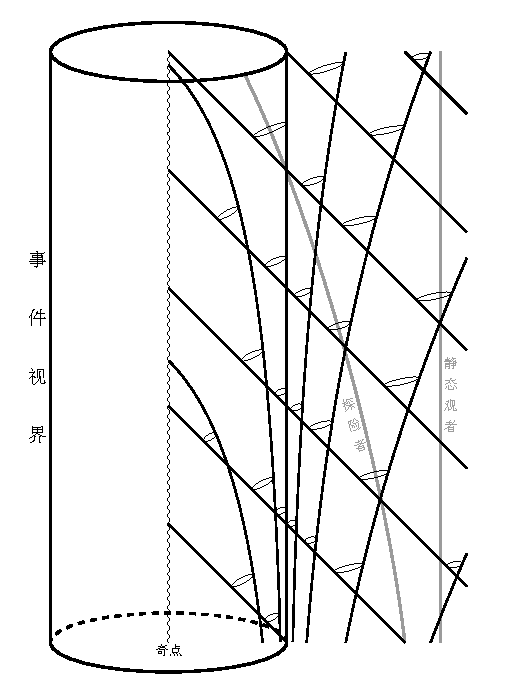
\includegraphics[width=.6\textwidth]{fig/chpt02/schBH.pdf}
    \caption{\small 静态黑洞 Eddington 图。绘制时积分常数均匀选取。可在格处画上椭圆,构成“妙脆角”,以代表微小未来光锥,或用“沙漏”表示完整光锥。}
\end{figure}
其中设有一个静态观者和一个位于 $\tilde t$-$r$ 平面的探险者。

\subsection{Kruskal 系}
Schwarzschild 系能保证 $g_{01}=0$ 而 Eddington 系不然。是否存在一个坐标系既能消除奇性,又能保持 $g_{01}=0$?

双曲线的渐近线相当于原点处的光锥 $C_N$。故对匀加速观者而言,信息不能从光锥另一侧逾越过来

故称\textbf{Rindler 视界}。

同理求出内、外向族分别为
\[
t=-\ln x+C_1,\quad t=\ln x+C_2.
\]
故可绘制如下图 。

注意,闵氏度规在 Rindler 系是有奇性的,因为其行列式 $g=-x^2$ 在 $x=0$ 处为零。可见,Rindler 系和闵氏系的相对地位,就像是 Schwarzschild 系或 Eddington 系和“更好”坐标系的相对地位。



因此上述类光测地线族其实“对应于”闵氏时空里的类光测地线族
\[
T=-X+C_1,\quad T=X+C_2.
\]

仿照这一思想,欲视类光测地线族为坐标网格(称为\textit{类光坐标})。

第  节中将双曲线、射线视作坐标线而衍生出 Rindler 坐标系,在 Rindler 图  里,这是在令
\eq{
v=t+\ln x,\quad u=t-\ln x.
}
度规表为 $\d s^2=-\e^{v-u}\d v\d u$。

而在闵氏图里是令
\eq{
V=T+X,\quad U=T-X,
}
或
\eq{
T=\frac{V+U}{2},\quad X=\frac{V-U}{2},
}
这有双曲函数的形式,而 $T,X$ 与 $t,x$ 的变换正是双曲函数,

故易知如下指数式
\eq{
V=\e^v>0,\quad U=-\e^{-u}<0.
}
度规现表为 $\d s^2=-\d V\d U$,不存在任何坐标奇性。

\begin{figure}[h!]
    \centering
    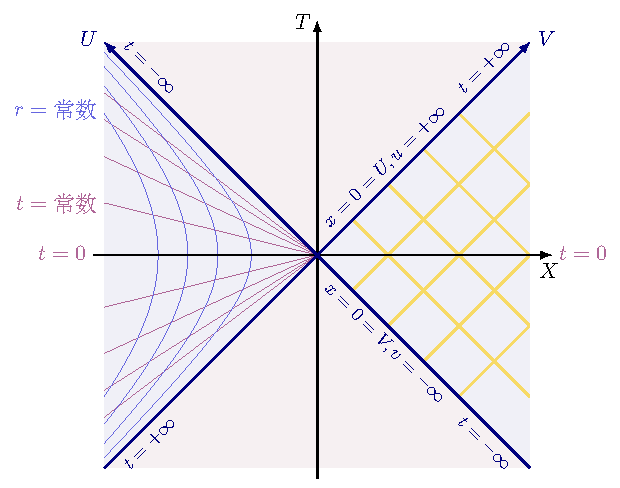
\includegraphics[width=.6\textwidth]{fig/chpt02/rindler.pdf}
    \caption{消除 Rindler 系的坐标奇性}
    \label{fig:rindlerIM}
\end{figure}
如图 \ref{fig:rindlerIM} 所示,则从直观上,闵氏时空图就像是把 Rindler 图 里竖直的 $x=0$ 从 $t=0$ 处向右“掰弯”成如光锥面一般的 Rindler 视界 $T^2=X^2$,即 $VU=0$,由上式知 $V,U$ 轴正方向如图 \ref{fig:rindlerIM}。图中蓝色双曲线代表等 $r$ 线,红色射线代表等 $t$ 线。可见,从 Rindler 图到闵氏图经历了如下过程:
\[
(t,x)\to(v,u)\to(V,U)\to(T,X).
\]
依葫芦画瓢地寻找“更好”坐标系。在超前 Eddington 系中,时间对角项在 $r=2M$ 为零,为消除奇性,只能借由超前变换所产生的非零时空交叉项,但我们并不想要交叉项。可见,必须使 $T,X$ 坐标的时间对角项非零。回到 Schwarzschild 系。不妨先研究 $r>2M$。$v,u$ 从类光测地线族产生,注意式 \eqref{dia_Sch} 与 $t=\pm r_*$ 相差常数,因此内、外向族分别给出
\eq{
v=t+r_*,\quad u=t-r_*.
}
由于 $r_*$ 作了超前变换,因此前者称\textit{超前类光坐标},后者称\textit{推迟类光坐标}。可见对 Rindler 时空来说其乌龟坐标是 $x_*=\ln x$,读者很容易验证这一点。度规在 $v,u$ 下表为
\[
\d s^2=-(1-2M/r)\d v\d u,
\]
沿用 $V,U$ 的指数形式但预留待定常数(只可与 $M$ 有关)以使最终的时间对角项非零\footnote{有种做法是填上 $1/\beta=4M$ 因子以约去指数求导出的系数,这样度规 \eqref{eq:kruskal} 中 ${32M^3}/{r}$ 变为 $2M/r$。}:
\eq{
V=\e^{\beta v}>0,\quad U=-\e^{-\beta u}<0.
}
只预留一个是考虑到对称性。进而度规表为
\[
\d s^2=-\beta^{-2} (1-2M/r) \e^{\beta(u-v)} \d V\d U,
\]
考虑到 $T,X$ 系只是 $V,U$ 系的旋转,我们可将其定义沿用至此,则 $-\d V\d U=-\d T^2+\d X^2$,进而保证无交叉项。现在的目标就是约掉 $(1-2M/r)$ 通分后所含因子 $(r-2M)$。这份任务只能交由 $\e^{\beta(u-v)}$,我们就要用 $r$ 表示它(由稳态条件可预料无 $t$)。注意 $u-v=-2r_*$,代入 $r_*$ 定义有
\[
\e^{\beta(u-v)}=\e^{-2\beta r}\left(\frac{2M}{r-2M}\right)^{4\beta M},
\]
说明应取 $\beta=1/4M$,则
\[
\d s^2=-\frac{32M^3}{r}\e^{-r/2M}\d V\d U=\frac{32M^3}{r}\e^{-r/2M}(-\d T^2+\d X^2).
\]
这里仍留有一个不能消除的时空奇点 $r=0$,与 Rindler 情况有所不同。综上,还原另外两个空间维度后,Schwarzschild 度规就表为
\eq{\label{eq:kruskal}
\d s^2=\frac{32M^3}{r}\e^{-r/2M}(-\d T^2+\d X^2)+r^2\d\Omega^2,
}
这里 $r$ 视作 $T,X$ 的函数,易知
\eq{
X^2-T^2=-VU=\e^{(v-u)/4M}=\left(\frac{r}{2M}-1\right)\e^{r/2M},
}
可用 Lambert 函数将其表为
\eq{\label{eq:r=T,X}
r=2M\operatorname{W}\left(\frac{X^2-T^2}{\e}\right)+2M.
}
这个坐标系称为 \textit{Kruskal 系}。我们再次按 $T,X$ 正交绘制 2 维时空图。$(-\d T^2+\d X^2)$ 形式的保留使类光测地线斜率仍为 $\pm 1$。实际上,像这样给原度规乘以一个正因子就称为 \textit{Weyl 重标度(rescaling)变换},简称 Weyl 变换,它能保留时空结构,故又称为\textit{共形(conformal)变换}。
\begin{figure}[h!]
    \centering
    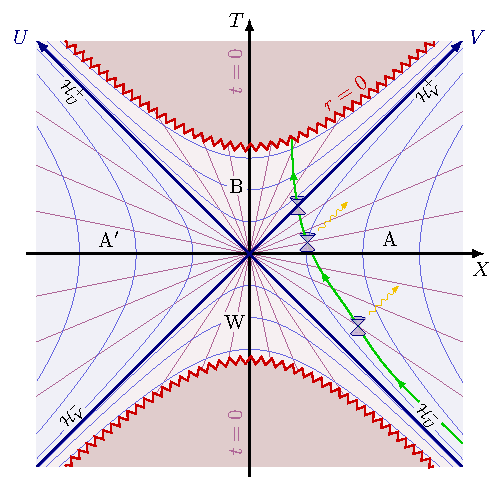
\includegraphics[width=.6\textwidth]{fig/chpt02/kruskal.pdf}
    \caption{Kruskal 延拓}
    \label{fig:kruskal}
\end{figure}
从图 \ref{fig:kruskal} 上可见,Kruskal 系也会“掰弯” Schwarzschild 时空的视界 $r=2M$,使之变为光锥面 $VU=0$。易知各坐标的取值分布同图 \ref{fig:rindlerIM} 相似。然而,我们只考虑了 $r>2M$ 的情况,在图上标记为开区域 \textit{A 区},对应 $V>0,U<0$。那 $r<2M$ 呢?Schwarzschild 系的 $r>2M$ 和 $r<2M$ 借超前 Eddington 系消除 $r=2M$ 坐标奇性。
从图上看,从 A 区任意点出发的内向类光线一定坠向 $V$ 正半轴,说明其代表事件视界,故可记作 $\H_V^+$。Kruskal 系也能消除坐标奇性,我们可越过视界来到上方,这里 $V,U>0$,说明我们自然地拓宽了 $V,U$ 的定义。为使 $U$ 为正,应定义
\eq{
V=\e^{v/4M}>0,\quad U=\e^{-u/4M}>0,
}
可验证度规仍表为 \eqref{eq:kruskal} 式。这里等 $r$ 线应无限延伸,因为等 $t$ 线从 $U$ 正半轴至 $V$ 正半轴遍历了所有 $t$ 值。一系列等 $r$ 线至多扫至时空奇点 $r=0\Leftrightarrow T^2-X^2=1$ 而无法越过,所扫区域里的任意类时、类光线确实都坠入奇点,说明其代表黑洞,称为 \textit{B 区}。可见,超前 Eddington 系覆盖了 $\mathrm{A}\cup\H_V^+\cup\mathrm{B}$,即整个 Schwarzschild 时空。奇点及其外部红色区域不属于时空。综上,A,B 区的坐标变换可整合为
\eq{
V=\e^{(r_*+t)/4M},\quad U=-\sgn(r-2M)\e^{(r_*-t)/4M}.
}
进而变换至 $T,X$ 可整合为
\eq{\begin{aligned}
    T&=\frac{\e^{r/4M}}{2}\sqrt{\abs{\frac{r}{2M}-1}} \left(\e^{t/4M}-\sgn(r-2M)\e^{t/4M}\right),\\
    X&=\frac{\e^{r/4M}}{2}\sqrt{\abs{\frac{r}{2M}-1}} \left(\e^{t/4M}+\sgn(r-2M)\e^{t/4M}\right).
\end{aligned}}
其仍形如双曲函数。若从 $T,X$ 做逆变换,易知 $r$ 仍满足 \eqref{eq:r=T,X} 式,而 $t$ 表为
\eq{
t=2M\ln\frac{X+T}{|X-T|},
}
形如反双曲正切函数。




使度规式  越过视界而自然地\textit{延拓(extend)}至内部,但即使如此也不能越过点 $r=0$,

直观上是因为我们已经覆盖了整个 $r>0$,而 $r<0$ 无意义。本节末会讲清延拓方法。




考虑到右加速观者和左加速观者不能相互交流,故可看作两个独立区域。



然而上图   只覆盖了闵氏时空图右边的类空区域。因此闵氏时空可以看作“Rindler 时空”(即 $x>0$ 部分)的\textit{延拓(extension)}。前文多次提及延拓这个词,通俗来讲,我们总想使坐标系尽可能覆盖得更广、更完整,且消除坐标奇性。而一旦变换坐标,甚至有可能推广新坐标的定义域,也就是延拓时空本身,且延拓后的时空还能包含坐标奇点,因为这时已无奇性。综上所述,无论 Schwarzschild 系   还是超前 Eddington 系 ,二者所对应的时空或许只是某个更大时空的\textit{子时空}。为此可想办法延拓它,直至一个可以证明不能再延拓的结果,称之为\textit{最大延拓(maximal extension)}。



若给 Rindler 图补上 $x<0$ 的部分




当然,仍有微妙区别:在 Rindler 图   中类光测地线无限延伸,而在闵氏图 \ref{fig:rindlerIM} 里这堆类光线并非如此。然而,使其延伸是很简单的:$V,U$ 可不按指数定义而自然延拓至整个 $\R^2$。


这就是用坐标系延拓时空。形象地说,本身或延拓后无限延伸的测地线称为\textit{完备的(complete)}。只有那种根本不能再继续延伸的测地线,才能叫\textit{不完备(incomplete)}。可见,不完备测地线表征了时空本身的不可延拓性(一旦延拓了就能完备),这时碰上的就并非坐标奇性了,而是实实在在的时空奇性,正如奇点那样。




这里第一步是转化至子时空



因而内外可视作独立区域

只限于 $r>0$


该式表明 Schwarzschild 度规可定义在一个比原来大得多的时空上,称其 \textit{Kruskal 延拓}。

,我们无法再继续延拓下去,因此 Kruskal 延拓是 Schwarzschild 时空的最大延拓。

2 维 Kruskal 延拓只是 $\R^2$ 的一个蝴蝶状子集



因而我们又称 Kruskal 延拓是\textit{共形平直}的。



将 Kruskal 延拓分为 4 个开区域,从右边开始,逆时针依次标记为 I,II,III,IV 区(后二者也有称 I$'$,II$'$ 的)。



其它 3 个区皆为 A 区延拓结果



可以预料,若对 Schwarzschild 系坐标时 $t$ 做推迟变换,即得超前 Eddington 系的时间反演坐标,故称\textit{推迟 Eddington 系},它描述的就是黑洞的反演:物质从视界穿出,物理现象朝着与黑洞性质相反的方向进行。从图上看,IV 区沿类时方向可以走向 A 区。物理学家将 IV 区打趣地称为\textit{白洞(white hole)},简称 \textit{W 区}。同理\textit{白洞视界}记 $\H_V^-,\H_U^-$。可见,推迟 Eddington 系覆盖了 $\mathrm{A}\cup\H_U^-\cup\mathrm{W}$。最后还有一个 III 区,从度规上看,其也是一个渐近平直视界外时空,而它亦可从 W 区穿出而坠入 B 区,鉴于相似性又称 III 区为 \textit{A$'$ 区},然而此二区域不可能有任何信息交流,即\textit{无因果联系},因为从 A 出发的任意类时或类光线都不能进入 A$'$,反之亦然。于是物理学家戏称 A$'$ 为另一独立的“宇宙”,二者互为\textit{平行宇宙(parallel universes)}。如果硬要说二者有“擦边性”的瓜葛,那只能在原点 $V,U=0$ 处。还原另二空间维度,它就是一个半径 $r=2M$ 的 2 维球面,称为\textit{虫洞(wormhole)}、\textit{喉(throat)}或\textit{分叉点(bifurcation)},以代表两个“宇宙”唯一可能但却不能通过的道路。这些概念是在全时空为真空的前提下所得,其物理实在性还须另做讨论。从初值问题的角度考虑,整个时空存在的可能性很小。

\section{Penrose 图}

\section{嵌入图与虫洞}
绘制虫洞的一个形象方法就是用嵌入图。


\section{引力坍缩}\label{sec:collapse}

星体演化

这些问题花了很长时间才理清,因为整体微分几何的流形语言是在场方程之后才发展完整的。

人们现在普遍认为星体\textit{引力坍缩(gravitational collapse)}的末日归宿就是黑洞。

进入黑洞的测地线会在有限固有时内碰上奇点而“断掉”,不可无限制地延伸下去,称作\textit{不可延测地线(inextendible geodesic)}。接近奇点的宏观观者会被差距强烈的潮汐力撕碎。

这种病态性质与高度的球对称性有关。Penrose 在 1965 年给出的\textit{奇性定理(singularity theorem)}中指出,耦合适当的物质并附加某些条件后,一定会出现不可延测地线,因而就产生了这么个奇点。奇性定理给出了两个重要猜想(conjecture)或者假设(hypothesis)。第一个是\textit{弱宇宙监督(weak cosmic censorship)假设}: 对于适当的物质方程组和一般物理意义的初始条件,奇点一定限制在黑洞区域内而“看不见”; 第二个是\textit{强(strong)宇宙监督假设}:解的奇性一定与其延拓遇到局部阻碍有关。后一个假设保证了动力学问题的唯一解必定是初始数据产生的经典时空,即\textit{经典决定性原理(Classical Newtonian determinism)}。如果抛弃条件的一般性,则这两个假设都不成立。Christodoulou 做出过标量场方程组的球对称解,其中的奇点就不在黑洞区域内,这样的时空就称作包含了\textit{裸(naked)奇点}。裸奇点很容易构造出来,比如直接令 $m<0$,但此时就不允许\textit{渐近平直(asymptotically flat)的 Cauchy 面}了,因而可能不太符合咱们的物理常识。这件事与所谓的\textit{正能量定理(positive mass theorem)}有关.


\section{RN 黑洞}

\section{黑洞热力学}

KN 黑洞

黑洞无毛猜想

\section{dS 与 AdS 时空}\label{sec:dS}



\section{轴对称时空}
    \subsection{Kerr 度规}
    \subsection{KN 度规}

\section{黑洞热力学}
\subsection{孤立视界}
\subsection{类光 Raychaudhuri 方程}
\subsection{信息论}


后 Newton 力学
